\documentclass[aspectratio=169,usenames,dvipsnames]{beamer}

\usetheme{default}  % You can choose any other theme you prefer

\title{03 - Algoritmos}
\author{Mateus Oliveira de Figueiredo}
\date{12/09/2023}

\usepackage{tikz}
\usepackage{multicol}
\usepackage{algorithm}
\usepackage{algpseudocode}
\usepackage{xcolor}
\usepackage[utf8]{inputenc}

\usepackage{pgfplots}
\DeclareUnicodeCharacter{2212}{−}
\usepgfplotslibrary{groupplots,dateplot}
\usetikzlibrary{patterns,shapes.arrows}
\pgfplotsset{compat=newest}

\begin{document}

\begin{frame}
\titlepage
\end{frame}

\begin{frame}
\frametitle{Problema}

\onslide<1->{
  \begin{block}{Problema}
    Dado um conjunto de pontos no  $\mathbb{R}^2$, encontrar o menor polígono convexo que contém todos os pontos.
  \end{block}
}
\begin{figure}
\begin{overprint}
  \onslide<2> \begin{center}
% This file was created with tikzplotlib v0.10.1.
\begin{tikzpicture}[scale=0.9]

\definecolor{darkslategray38}{RGB}{38,38,38}
\definecolor{lightgray204}{RGB}{204,204,204}
\definecolor{steelblue76114176}{RGB}{76,114,176}

\begin{axis}[
axis line style={lightgray204},
hide x axis,
hide y axis,
tick align=outside,
x grid style={lightgray204},
xmajorticks=false,
xmin=0.0669367338947019, xmax=0.894111789939664,
xtick style={color=darkslategray38},
y grid style={lightgray204},
ymajorticks=false,
ymin=-0.0362471743023485, ymax=1.03274876525929,
ytick style={color=darkslategray38}
]
\addplot [draw=steelblue76114176, fill=steelblue76114176, mark=*, only marks]
table{%
x  y
0.346517060199814 0.201667385571862
0.110198245014805 0.710446973195645
0.674196381095166 0.49152149407659
0.30956117598126 0.80506608165215
0.271019344924566 0.98415804073376
0.636154602711755 0.693008958661624
0.384544745815431 0.621686927298183
0.613069361293463 0.536676532843469
0.515872695614497 0.0123435502231805
0.856512923755802 0.429885536698643
0.794765500051758 0.575905243509799
0.104535600078564 0.331190264339077
0.698107527894101 0.591287819523784
0.652331867510728 0.829843579751645
0.776100950068952 0.0753407526360956
0.359461819254946 0.832493157115646
0.234215740614521 0.440279847038206
0.474800803395323 0.180277096021146
0.478504950884847 0.867281705269675
0.434092000130053 0.504691515965982
0.640277876553855 0.402360080889356
};
\end{axis}

\end{tikzpicture}

\end{center}
  \onslide<3> % This file was created with tikzplotlib v0.10.1.
\begin{center}
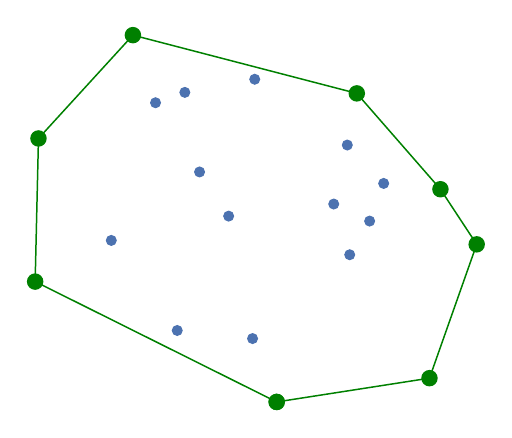
\begin{tikzpicture}[scale=0.9]

\definecolor{darkslategray38}{RGB}{38,38,38}
\definecolor{green}{RGB}{0,128,0}
\definecolor{lightgray204}{RGB}{204,204,204}
\definecolor{steelblue76114176}{RGB}{76,114,176}

\begin{axis}[
axis line style={lightgray204},
hide x axis,
hide y axis,
tick align=outside,
x grid style={lightgray204},
xmajorticks=false,
xmin=0.0669367338947019, xmax=0.894111789939664,
xtick style={color=darkslategray38},
y grid style={lightgray204},
ymajorticks=false,
ymin=-0.0362471743023485, ymax=1.03274876525929,
ytick style={color=darkslategray38}
]
\addplot [draw=steelblue76114176, fill=steelblue76114176, mark=*, only marks]
table{%
x  y
0.346517060199814 0.201667385571862
0.110198245014805 0.710446973195645
0.674196381095166 0.49152149407659
0.30956117598126 0.80506608165215
0.271019344924566 0.98415804073376
0.636154602711755 0.693008958661624
0.384544745815431 0.621686927298183
0.613069361293463 0.536676532843469
0.515872695614497 0.0123435502231805
0.856512923755802 0.429885536698643
0.794765500051758 0.575905243509799
0.104535600078564 0.331190264339077
0.698107527894101 0.591287819523784
0.652331867510728 0.829843579751645
0.776100950068952 0.0753407526360956
0.359461819254946 0.832493157115646
0.234215740614521 0.440279847038206
0.474800803395323 0.180277096021146
0.478504950884847 0.867281705269675
0.434092000130053 0.504691515965982
0.640277876553855 0.402360080889356
};
\addplot [semithick, green, mark=*, mark size=3, mark options={solid}]
table {%
0.515872695614497 0.0123435502231805
0.776100950068952 0.0753407526360956
0.856512923755802 0.429885536698643
0.794765500051758 0.575905243509799
0.652331867510728 0.829843579751645
0.271019344924566 0.98415804073376
0.110198245014805 0.710446973195645
0.104535600078564 0.331190264339077
0.515872695614497 0.0123435502231805
};
\end{axis}

\end{tikzpicture}
\end{center}
\end{overprint}
\end{figure}

\end{frame}

\begin{frame}{Algoritmos}
      Três algoritmos implementados:
      \begin{itemize}
        \item Algoritmo Triângulos: $O(n^4)$
        \item Algoritmo Segmentos: $O(n^3)$
        \item Algoritmo de Jarvis: $O(hn)$
      \end{itemize}
\end{frame}

\begin{frame}{Algoritmo Triângulos}

  % Add centralized figure
  \begin{center}
    \begin{figure}
      \begin{overprint}
        \onslide<1>\begin{center}
% This file was created with tikzplotlib v0.10.1.
\begin{tikzpicture}[scale=0.9]

\definecolor{darkslategray38}{RGB}{38,38,38}
\definecolor{lightgray204}{RGB}{204,204,204}
\definecolor{steelblue76114176}{RGB}{76,114,176}

\begin{axis}[
axis line style={lightgray204},
hide x axis,
hide y axis,
tick align=outside,
x grid style={lightgray204},
xmajorticks=false,
xmin=0.0669367338947019, xmax=0.894111789939664,
xtick style={color=darkslategray38},
y grid style={lightgray204},
ymajorticks=false,
ymin=-0.0362471743023485, ymax=1.03274876525929,
ytick style={color=darkslategray38}
]
\addplot [draw=steelblue76114176, fill=steelblue76114176, mark=*, only marks]
table{%
x  y
0.346517060199814 0.201667385571862
0.110198245014805 0.710446973195645
0.674196381095166 0.49152149407659
0.30956117598126 0.80506608165215
0.271019344924566 0.98415804073376
0.636154602711755 0.693008958661624
0.384544745815431 0.621686927298183
0.613069361293463 0.536676532843469
0.515872695614497 0.0123435502231805
0.856512923755802 0.429885536698643
0.794765500051758 0.575905243509799
0.104535600078564 0.331190264339077
0.698107527894101 0.591287819523784
0.652331867510728 0.829843579751645
0.776100950068952 0.0753407526360956
0.359461819254946 0.832493157115646
0.234215740614521 0.440279847038206
0.474800803395323 0.180277096021146
0.478504950884847 0.867281705269675
0.434092000130053 0.504691515965982
0.640277876553855 0.402360080889356
};
\end{axis}

\end{tikzpicture}

\end{center}
        \onslide<2>\begin{center}
% This file was created with tikzplotlib v0.10.1.
\begin{tikzpicture}[scale=0.9]

\definecolor{darkslategray38}{RGB}{38,38,38}
\definecolor{lightgray204}{RGB}{204,204,204}
\definecolor{steelblue76114176}{RGB}{76,114,176}

\begin{axis}[
axis line style={lightgray204},
hide x axis,
hide y axis,
tick align=outside,
x grid style={lightgray204},
xmajorticks=false,
xmin=0.0669367338947019, xmax=0.894111789939664,
xtick style={color=darkslategray38},
y grid style={lightgray204},
ymajorticks=false,
ymin=-0.0362471743023485, ymax=1.03274876525929,
ytick style={color=darkslategray38}
]
\addplot [draw=steelblue76114176, fill=steelblue76114176, mark=*, only marks]
table{%
x  y
0.346517060199814 0.201667385571862
0.110198245014805 0.710446973195645
0.674196381095166 0.49152149407659
0.30956117598126 0.80506608165215
0.271019344924566 0.98415804073376
0.636154602711755 0.693008958661624
0.384544745815431 0.621686927298183
0.613069361293463 0.536676532843469
0.515872695614497 0.0123435502231805
0.856512923755802 0.429885536698643
0.794765500051758 0.575905243509799
0.104535600078564 0.331190264339077
0.698107527894101 0.591287819523784
0.652331867510728 0.829843579751645
0.776100950068952 0.0753407526360956
0.359461819254946 0.832493157115646
0.234215740614521 0.440279847038206
0.474800803395323 0.180277096021146
0.478504950884847 0.867281705269675
0.434092000130053 0.504691515965982
0.640277876553855 0.402360080889356
};
\addplot [semithick, black]
table {%
0.636154602711755 0.693008958661624
0.234215740614521 0.440279847038206
0.640277876553855 0.402360080889356
0.636154602711755 0.693008958661624
};
\end{axis}

\end{tikzpicture}

\end{center}
        \onslide<3>% This file was created with tikzplotlib v0.10.1.
\begin{tikzpicture}

\definecolor{darkslategray38}{RGB}{38,38,38}
\definecolor{lightgray204}{RGB}{204,204,204}
\definecolor{steelblue76114176}{RGB}{76,114,176}

\begin{axis}[
axis line style={lightgray204},
hide x axis,
hide y axis,
tick align=outside,
x grid style={lightgray204},
xmajorticks=false,
xmin=0.0669367338947019, xmax=0.894111789939664,
xtick style={color=darkslategray38},
y grid style={lightgray204},
ymajorticks=false,
ymin=-0.0362471743023485, ymax=1.03274876525929,
ytick style={color=darkslategray38}
]
\addplot [draw=steelblue76114176, fill=steelblue76114176, mark=*, only marks]
table{%
x  y
0.346517060199814 0.201667385571862
0.110198245014805 0.710446973195645
0.674196381095166 0.49152149407659
0.30956117598126 0.80506608165215
0.271019344924566 0.98415804073376
0.636154602711755 0.693008958661624
0.384544745815431 0.621686927298183
0.613069361293463 0.536676532843469
0.515872695614497 0.0123435502231805
0.856512923755802 0.429885536698643
0.794765500051758 0.575905243509799
0.104535600078564 0.331190264339077
0.698107527894101 0.591287819523784
0.652331867510728 0.829843579751645
0.776100950068952 0.0753407526360956
0.359461819254946 0.832493157115646
0.234215740614521 0.440279847038206
0.474800803395323 0.180277096021146
0.478504950884847 0.867281705269675
0.434092000130053 0.504691515965982
0.640277876553855 0.402360080889356
};
\addplot [draw=red, fill=red, mark=*, only marks]
table{%
x  y
0.613069361293463 0.536676532843469
0.434092000130053 0.504691515965982
};
\addplot [semithick, black]
table {%
0.636154602711755 0.693008958661624
0.234215740614521 0.440279847038206
0.640277876553855 0.402360080889356
0.636154602711755 0.693008958661624
};
\end{axis}

\end{tikzpicture}

        \onslide<4>\begin{center}
% This file was created with tikzplotlib v0.10.1.
\begin{tikzpicture}[scale=0.9]

\definecolor{darkslategray38}{RGB}{38,38,38}
\definecolor{lightgray204}{RGB}{204,204,204}
\definecolor{steelblue76114176}{RGB}{76,114,176}

\begin{axis}[
axis line style={lightgray204},
hide x axis,
hide y axis,
tick align=outside,
x grid style={lightgray204},
xmajorticks=false,
xmin=0.0669367338947019, xmax=0.894111789939664,
xtick style={color=darkslategray38},
y grid style={lightgray204},
ymajorticks=false,
ymin=-0.0362471743023485, ymax=1.03274876525929,
ytick style={color=darkslategray38}
]
\addplot [draw=steelblue76114176, fill=steelblue76114176, mark=*, only marks]
table{%
x  y
0.346517060199814 0.201667385571862
0.110198245014805 0.710446973195645
0.674196381095166 0.49152149407659
0.30956117598126 0.80506608165215
0.271019344924566 0.98415804073376
0.636154602711755 0.693008958661624
0.384544745815431 0.621686927298183
0.613069361293463 0.536676532843469
0.515872695614497 0.0123435502231805
0.856512923755802 0.429885536698643
0.794765500051758 0.575905243509799
0.104535600078564 0.331190264339077
0.698107527894101 0.591287819523784
0.652331867510728 0.829843579751645
0.776100950068952 0.0753407526360956
0.359461819254946 0.832493157115646
0.234215740614521 0.440279847038206
0.474800803395323 0.180277096021146
0.478504950884847 0.867281705269675
0.434092000130053 0.504691515965982
0.640277876553855 0.402360080889356
};
\addplot [draw=red, fill=red, mark=*, only marks]
table{%
x  y
0.613069361293463 0.536676532843469
0.434092000130053 0.504691515965982
};
\addplot [semithick, black]
table {%
0.104535600078564 0.331190264339077
0.474800803395323 0.180277096021146
0.478504950884847 0.867281705269675
0.104535600078564 0.331190264339077
};
\end{axis}

\end{tikzpicture}

\end{center}
        \onslide<5>% This file was created with tikzplotlib v0.10.1.
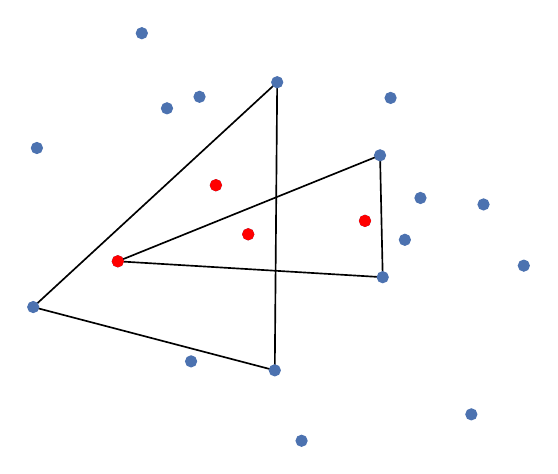
\begin{tikzpicture}

\definecolor{darkslategray38}{RGB}{38,38,38}
\definecolor{lightgray204}{RGB}{204,204,204}
\definecolor{steelblue76114176}{RGB}{76,114,176}

\begin{axis}[
axis line style={lightgray204},
hide x axis,
hide y axis,
tick align=outside,
x grid style={lightgray204},
xmajorticks=false,
xmin=0.0669367338947019, xmax=0.894111789939664,
xtick style={color=darkslategray38},
y grid style={lightgray204},
ymajorticks=false,
ymin=-0.0362471743023485, ymax=1.03274876525929,
ytick style={color=darkslategray38}
]
\addplot [draw=steelblue76114176, fill=steelblue76114176, mark=*, only marks]
table{%
x  y
0.346517060199814 0.201667385571862
0.110198245014805 0.710446973195645
0.674196381095166 0.49152149407659
0.30956117598126 0.80506608165215
0.271019344924566 0.98415804073376
0.636154602711755 0.693008958661624
0.384544745815431 0.621686927298183
0.613069361293463 0.536676532843469
0.515872695614497 0.0123435502231805
0.856512923755802 0.429885536698643
0.794765500051758 0.575905243509799
0.104535600078564 0.331190264339077
0.698107527894101 0.591287819523784
0.652331867510728 0.829843579751645
0.776100950068952 0.0753407526360956
0.359461819254946 0.832493157115646
0.234215740614521 0.440279847038206
0.474800803395323 0.180277096021146
0.478504950884847 0.867281705269675
0.434092000130053 0.504691515965982
0.640277876553855 0.402360080889356
};
\addplot [draw=red, fill=red, mark=*, only marks]
table{%
x  y
0.613069361293463 0.536676532843469
0.434092000130053 0.504691515965982
};
\addplot [draw=red, fill=red, mark=*, only marks]
table{%
x  y
0.384544745815431 0.621686927298183
0.234215740614521 0.440279847038206
};
\addplot [semithick, black]
table {%
0.636154602711755 0.693008958661624
0.234215740614521 0.440279847038206
0.640277876553855 0.402360080889356
0.636154602711755 0.693008958661624
};
\addplot [semithick, black]
table {%
0.104535600078564 0.331190264339077
0.474800803395323 0.180277096021146
0.478504950884847 0.867281705269675
0.104535600078564 0.331190264339077
};
\end{axis}

\end{tikzpicture}

        \onslide<6->% This file was created with tikzplotlib v0.10.1.
\begin{tikzpicture}[scale=0.9]

\definecolor{darkslategray38}{RGB}{38,38,38}
\definecolor{lightgray204}{RGB}{204,204,204}
\definecolor{steelblue76114176}{RGB}{76,114,176}

\begin{axis}[
axis line style={lightgray204},
hide x axis,
hide y axis,
tick align=outside,
x grid style={lightgray204},
xmajorticks=false,
xmin=0.0669367338947019, xmax=0.894111789939664,
xtick style={color=darkslategray38},
y grid style={lightgray204},
ymajorticks=false,
ymin=-0.0362471743023485, ymax=1.03274876525929,
ytick style={color=darkslategray38}
]
\addplot [draw=steelblue76114176, fill=steelblue76114176, mark=*, only marks]
table{%
x  y
0.346517060199814 0.201667385571862
0.110198245014805 0.710446973195645
0.674196381095166 0.49152149407659
0.30956117598126 0.80506608165215
0.271019344924566 0.98415804073376
0.636154602711755 0.693008958661624
0.384544745815431 0.621686927298183
0.613069361293463 0.536676532843469
0.515872695614497 0.0123435502231805
0.856512923755802 0.429885536698643
0.794765500051758 0.575905243509799
0.104535600078564 0.331190264339077
0.698107527894101 0.591287819523784
0.652331867510728 0.829843579751645
0.776100950068952 0.0753407526360956
0.359461819254946 0.832493157115646
0.234215740614521 0.440279847038206
0.474800803395323 0.180277096021146
0.478504950884847 0.867281705269675
0.434092000130053 0.504691515965982
0.640277876553855 0.402360080889356
};
\addplot [draw=red, fill=red, mark=*, only marks]
table{%
x  y
0.346517060199814 0.201667385571862
0.674196381095166 0.49152149407659
0.30956117598126 0.80506608165215
0.636154602711755 0.693008958661624
0.384544745815431 0.621686927298183
0.613069361293463 0.536676532843469
0.698107527894101 0.591287819523784
0.359461819254946 0.832493157115646
0.234215740614521 0.440279847038206
0.474800803395323 0.180277096021146
0.478504950884847 0.867281705269675
0.434092000130053 0.504691515965982
0.640277876553855 0.402360080889356
};
\end{axis}

\end{tikzpicture}

      \end{overprint}
    \end{figure}
  \end{center}

  \begin{overprint}
    \onslide<6>{
      \begin{equation}
        \text{Custo} = \underbrace{O(n^3)}_{\text{Triângulos}} \times \underbrace{O(n)}_{\text{Pontos dentro}} +\underbrace{O(nlog(n))}_{\text{Ordenar pontos}} = O(n^4)
      \end{equation}
    }
  \end{overprint}
\end{frame}

\begin{frame}{Algoritmo Segmentos}
  % Add centralized figure
  \begin{center}
    \begin{figure}
      \begin{overprint}
        \onslide<1>% This file was created with tikzplotlib v0.10.1.
\begin{tikzpicture}[scale=0.9]

\definecolor{darkslategray38}{RGB}{38,38,38}
\definecolor{lightgray204}{RGB}{204,204,204}
\definecolor{steelblue76114176}{RGB}{76,114,176}

\begin{axis}[
axis line style={lightgray204},
hide x axis,
hide y axis,
tick align=outside,
x grid style={lightgray204},
xmajorticks=false,
xmin=0.0669367338947019, xmax=0.894111789939664,
xtick style={color=darkslategray38},
y grid style={lightgray204},
ymajorticks=false,
ymin=-0.0362471743023485, ymax=1.03274876525929,
ytick style={color=darkslategray38}
]
\addplot [draw=steelblue76114176, fill=steelblue76114176, mark=*, only marks]
table{%
x  y
0.346517060199814 0.201667385571862
0.110198245014805 0.710446973195645
0.674196381095166 0.49152149407659
0.30956117598126 0.80506608165215
0.271019344924566 0.98415804073376
0.636154602711755 0.693008958661624
0.384544745815431 0.621686927298183
0.613069361293463 0.536676532843469
0.515872695614497 0.0123435502231805
0.856512923755802 0.429885536698643
0.794765500051758 0.575905243509799
0.104535600078564 0.331190264339077
0.698107527894101 0.591287819523784
0.652331867510728 0.829843579751645
0.776100950068952 0.0753407526360956
0.359461819254946 0.832493157115646
0.234215740614521 0.440279847038206
0.474800803395323 0.180277096021146
0.478504950884847 0.867281705269675
0.434092000130053 0.504691515965982
0.640277876553855 0.402360080889356
};
\addplot [draw=none, draw=white, fill=white, mark=*]
table{%
x  y
0 -0.5
0.13260155 -0.5
0.259789935392427 -0.447316845794121
0.353553390593274 -0.353553390593274
0.447316845794121 -0.259789935392427
0.5 -0.13260155
0.5 0
0.5 0.13260155
0.447316845794121 0.259789935392427
0.353553390593274 0.353553390593274
0.259789935392427 0.447316845794121
0.13260155 0.5
0 0.5
-0.13260155 0.5
-0.259789935392427 0.447316845794121
-0.353553390593274 0.353553390593274
-0.447316845794121 0.259789935392427
-0.5 0.13260155
-0.5 0
-0.5 -0.13260155
-0.447316845794121 -0.259789935392427
-0.353553390593274 -0.353553390593274
-0.259789935392427 -0.447316845794121
-0.13260155 -0.5
0 -0.5
0 -0.5
};
\end{axis}

\end{tikzpicture}

        \onslide<2->% This file was created with tikzplotlib v0.10.1.
\begin{tikzpicture}

\definecolor{darkslategray38}{RGB}{38,38,38}
\definecolor{forestgreen}{RGB}{34,139,34}
\definecolor{lightgray204}{RGB}{204,204,204}
\definecolor{steelblue76114176}{RGB}{76,114,176}

\begin{axis}[
axis line style={lightgray204},
hide x axis,
hide y axis,
tick align=outside,
x grid style={lightgray204},
xmajorticks=false,
xmin=0.0669367338947019, xmax=0.894111789939664,
xtick style={color=darkslategray38},
y grid style={lightgray204},
ymajorticks=false,
ymin=-0.0362471743023485, ymax=1.03274876525929,
ytick style={color=darkslategray38}
]
\addplot [draw=steelblue76114176, fill=steelblue76114176, mark=*, only marks]
table{%
x  y
0.346517060199814 0.201667385571862
0.110198245014805 0.710446973195645
0.674196381095166 0.49152149407659
0.30956117598126 0.80506608165215
0.271019344924566 0.98415804073376
0.636154602711755 0.693008958661624
0.384544745815431 0.621686927298183
0.613069361293463 0.536676532843469
0.515872695614497 0.0123435502231805
0.856512923755802 0.429885536698643
0.794765500051758 0.575905243509799
0.104535600078564 0.331190264339077
0.698107527894101 0.591287819523784
0.652331867510728 0.829843579751645
0.776100950068952 0.0753407526360956
0.359461819254946 0.832493157115646
0.234215740614521 0.440279847038206
0.474800803395323 0.180277096021146
0.478504950884847 0.867281705269675
0.434092000130053 0.504691515965982
0.640277876553855 0.402360080889356
};
\addplot [draw=none, draw=white, fill=white, mark=*]
table{%
x  y
0 -0.5
0.13260155 -0.5
0.259789935392427 -0.447316845794121
0.353553390593274 -0.353553390593274
0.447316845794121 -0.259789935392427
0.5 -0.13260155
0.5 0
0.5 0.13260155
0.447316845794121 0.259789935392427
0.353553390593274 0.353553390593274
0.259789935392427 0.447316845794121
0.13260155 0.5
0 0.5
-0.13260155 0.5
-0.259789935392427 0.447316845794121
-0.353553390593274 0.353553390593274
-0.447316845794121 0.259789935392427
-0.5 0.13260155
-0.5 0
-0.5 -0.13260155
-0.447316845794121 -0.259789935392427
-0.353553390593274 -0.353553390593274
-0.259789935392427 -0.447316845794121
-0.13260155 -0.5
0 -0.5
0 -0.5
};
\addplot [very thick, forestgreen]
table {%
0.515872695614497 0.0123435502231805
0.776100950068952 0.0753407526360956
};
\addplot [very thick, red]
table {%
0.346517060199814 0.201667385571862
0.434092000130053 0.504691515965982
};
\end{axis}

\end{tikzpicture}

      \end{overprint}
    \end{figure}
  \end{center}

  \begin{overprint}
    \onslide<3>{
      \begin{equation}
        \text{Custo} = \underbrace{O(n^2)}_{\text{Segmentos}} \times \underbrace{O(n)}_{\text{CCW Pontos}} + \underbrace{O(nlog(n))}_{\text{Ordenar pontos}} = O(n^3)
      \end{equation}
    }
  \end{overprint}
\end{frame}

\begin{frame}{Algoritmo Jarvis}
  % Add centralized figure
  \begin{center}
    \begin{figure}
      \begin{overprint}
        \onslide<1>\begin{center}
% This file was created with tikzplotlib v0.10.1.
\begin{tikzpicture}[scale=0.9]

\definecolor{darkslategray38}{RGB}{38,38,38}
\definecolor{lightgray204}{RGB}{204,204,204}
\definecolor{steelblue76114176}{RGB}{76,114,176}

\begin{axis}[
axis line style={lightgray204},
hide x axis,
hide y axis,
tick align=outside,
x grid style={lightgray204},
xmajorticks=false,
xmin=0.0669367338947019, xmax=0.894111789939664,
xtick style={color=darkslategray38},
y grid style={lightgray204},
ymajorticks=false,
ymin=-0.0362471743023485, ymax=1.03274876525929,
ytick style={color=darkslategray38}
]
\addplot [draw=steelblue76114176, fill=steelblue76114176, mark=*, only marks]
table{%
x  y
0.346517060199814 0.201667385571862
0.110198245014805 0.710446973195645
0.674196381095166 0.49152149407659
0.30956117598126 0.80506608165215
0.271019344924566 0.98415804073376
0.636154602711755 0.693008958661624
0.384544745815431 0.621686927298183
0.613069361293463 0.536676532843469
0.515872695614497 0.0123435502231805
0.856512923755802 0.429885536698643
0.794765500051758 0.575905243509799
0.104535600078564 0.331190264339077
0.698107527894101 0.591287819523784
0.652331867510728 0.829843579751645
0.776100950068952 0.0753407526360956
0.359461819254946 0.832493157115646
0.234215740614521 0.440279847038206
0.474800803395323 0.180277096021146
0.478504950884847 0.867281705269675
0.434092000130053 0.504691515965982
0.640277876553855 0.402360080889356
};
\end{axis}

\end{tikzpicture}

\end{center}
        \onslide<2>\begin{center}
% This file was created with tikzplotlib v0.10.1.
\begin{tikzpicture}[scale=0.9]

\definecolor{darkslategray38}{RGB}{38,38,38}
\definecolor{lightgray204}{RGB}{204,204,204}
\definecolor{steelblue76114176}{RGB}{76,114,176}

\begin{axis}[
axis line style={lightgray204},
hide x axis,
hide y axis,
tick align=outside,
x grid style={lightgray204},
xmajorticks=false,
xmin=0.0669367338947019, xmax=0.894111789939664,
xtick style={color=darkslategray38},
y grid style={lightgray204},
ymajorticks=false,
ymin=-0.0362471743023485, ymax=1.03274876525929,
ytick style={color=darkslategray38}
]
\addplot [semithick, white, mark=*, mark size=3, mark options={solid}]
table {%
0.515872695614497 0.0123435502231805
0.776100950068952 0.0753407526360956
0.856512923755802 0.429885536698643
0.794765500051758 0.575905243509799
0.652331867510728 0.829843579751645
0.271019344924566 0.98415804073376
0.110198245014805 0.710446973195645
0.104535600078564 0.331190264339077
};
\addplot [draw=steelblue76114176, fill=steelblue76114176, mark=*, only marks]
table{%
x  y
0.346517060199814 0.201667385571862
0.110198245014805 0.710446973195645
0.674196381095166 0.49152149407659
0.30956117598126 0.80506608165215
0.271019344924566 0.98415804073376
0.636154602711755 0.693008958661624
0.384544745815431 0.621686927298183
0.613069361293463 0.536676532843469
0.515872695614497 0.0123435502231805
0.856512923755802 0.429885536698643
0.794765500051758 0.575905243509799
0.104535600078564 0.331190264339077
0.698107527894101 0.591287819523784
0.652331867510728 0.829843579751645
0.776100950068952 0.0753407526360956
0.359461819254946 0.832493157115646
0.234215740614521 0.440279847038206
0.474800803395323 0.180277096021146
0.478504950884847 0.867281705269675
0.434092000130053 0.504691515965982
0.640277876553855 0.402360080889356
};
\addplot [semithick, black, mark=*, mark size=3, mark options={solid}]
table {%
0.104535600078564 0.0123435502231805
};
\draw (axis cs:0.104535600078564,0.0123435502231805) node[
  scale=0.6,
  anchor=south west,
  text=darkslategray38,
  rotate=0.0
]{$(x_{min}, y_{min})$};
\end{axis}

\end{tikzpicture}

\end{center}
        \onslide<3>\begin{center}
% This file was created with tikzplotlib v0.10.1.
\begin{tikzpicture}[scale=0.9]

\definecolor{darkslategray38}{RGB}{38,38,38}
\definecolor{green}{RGB}{0,128,0}
\definecolor{lightgray204}{RGB}{204,204,204}
\definecolor{steelblue76114176}{RGB}{76,114,176}

\begin{axis}[
axis line style={lightgray204},
hide x axis,
hide y axis,
tick align=outside,
x grid style={lightgray204},
xmajorticks=false,
xmin=0.0669367338947019, xmax=0.894111789939664,
xtick style={color=darkslategray38},
y grid style={lightgray204},
ymajorticks=false,
ymin=-0.0362471743023485, ymax=1.03274876525929,
ytick style={color=darkslategray38}
]
\addplot [draw=steelblue76114176, fill=steelblue76114176, mark=*, only marks]
table{%
x  y
0.346517060199814 0.201667385571862
0.110198245014805 0.710446973195645
0.674196381095166 0.49152149407659
0.30956117598126 0.80506608165215
0.271019344924566 0.98415804073376
0.636154602711755 0.693008958661624
0.384544745815431 0.621686927298183
0.613069361293463 0.536676532843469
0.515872695614497 0.0123435502231805
0.856512923755802 0.429885536698643
0.794765500051758 0.575905243509799
0.104535600078564 0.331190264339077
0.698107527894101 0.591287819523784
0.652331867510728 0.829843579751645
0.776100950068952 0.0753407526360956
0.359461819254946 0.832493157115646
0.234215740614521 0.440279847038206
0.474800803395323 0.180277096021146
0.478504950884847 0.867281705269675
0.434092000130053 0.504691515965982
0.640277876553855 0.402360080889356
};
\addplot [semithick, black, mark=*, mark size=3, mark options={solid}]
table {%
0.104535600078564 0.0123435502231805
};
\addplot [semithick, green, mark=*, mark size=3, mark options={solid}]
table {%
0.515872695614497 0.0123435502231805
};
\draw (axis cs:0.104535600078564,0.0123435502231805) node[
  scale=0.6,
  anchor=south west,
  text=darkslategray38,
  rotate=0.0
]{$(x_{min}, y_{min})$};
\end{axis}

\end{tikzpicture}

\end{center}
        \onslide<4>% This file was created with tikzplotlib v0.10.1.
\begin{tikzpicture}

\definecolor{darkslategray38}{RGB}{38,38,38}
\definecolor{green}{RGB}{0,128,0}
\definecolor{lightgray204}{RGB}{204,204,204}
\definecolor{steelblue76114176}{RGB}{76,114,176}

\begin{axis}[
axis line style={lightgray204},
hide x axis,
hide y axis,
tick align=outside,
x grid style={lightgray204},
xmajorticks=false,
xmin=0.0669367338947019, xmax=0.894111789939664,
xtick style={color=darkslategray38},
y grid style={lightgray204},
ymajorticks=false,
ymin=-0.0362471743023485, ymax=1.03274876525929,
ytick style={color=darkslategray38}
]
\addplot [draw=steelblue76114176, fill=steelblue76114176, mark=*, only marks]
table{%
x  y
0.346517060199814 0.201667385571862
0.110198245014805 0.710446973195645
0.674196381095166 0.49152149407659
0.30956117598126 0.80506608165215
0.271019344924566 0.98415804073376
0.636154602711755 0.693008958661624
0.384544745815431 0.621686927298183
0.613069361293463 0.536676532843469
0.515872695614497 0.0123435502231805
0.856512923755802 0.429885536698643
0.794765500051758 0.575905243509799
0.104535600078564 0.331190264339077
0.698107527894101 0.591287819523784
0.652331867510728 0.829843579751645
0.776100950068952 0.0753407526360956
0.359461819254946 0.832493157115646
0.234215740614521 0.440279847038206
0.474800803395323 0.180277096021146
0.478504950884847 0.867281705269675
0.434092000130053 0.504691515965982
0.640277876553855 0.402360080889356
};
\addplot [semithick, black, mark=*, mark size=3, mark options={solid}]
table {%
0.104535600078564 0.0123435502231805
};
\addplot [semithick, green, mark=*, mark size=3, mark options={solid}]
table {%
0.515872695614497 0.0123435502231805
};
\addplot [semithick, green, mark=*, mark size=3, mark options={solid}]
table {%
0.515872695614497 0.0123435502231805
0.776100950068952 0.0753407526360956
};
\draw (axis cs:0.104535600078564,0.0123435502231805) node[
  scale=0.6,
  anchor=south west,
  text=darkslategray38,
  rotate=0.0
]{$(x_{min}, y_{min})$};
\end{axis}

\end{tikzpicture}

        \onslide<5>% This file was created with tikzplotlib v0.10.1.
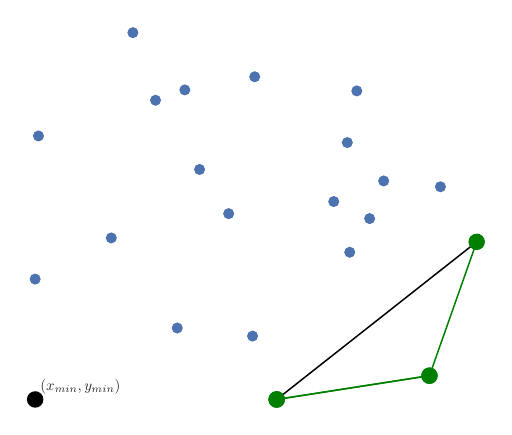
\begin{tikzpicture}[scale=0.9]

\definecolor{darkslategray38}{RGB}{38,38,38}
\definecolor{green}{RGB}{0,128,0}
\definecolor{lightgray204}{RGB}{204,204,204}
\definecolor{steelblue76114176}{RGB}{76,114,176}

\begin{axis}[
axis line style={lightgray204},
hide x axis,
hide y axis,
tick align=outside,
x grid style={lightgray204},
xmajorticks=false,
xmin=0.0669367338947019, xmax=0.894111789939664,
xtick style={color=darkslategray38},
y grid style={lightgray204},
ymajorticks=false,
ymin=-0.0362471743023485, ymax=1.03274876525929,
ytick style={color=darkslategray38}
]
\addplot [draw=steelblue76114176, fill=steelblue76114176, mark=*, only marks]
table{%
x  y
0.346517060199814 0.201667385571862
0.110198245014805 0.710446973195645
0.674196381095166 0.49152149407659
0.30956117598126 0.80506608165215
0.271019344924566 0.98415804073376
0.636154602711755 0.693008958661624
0.384544745815431 0.621686927298183
0.613069361293463 0.536676532843469
0.515872695614497 0.0123435502231805
0.856512923755802 0.429885536698643
0.794765500051758 0.575905243509799
0.104535600078564 0.331190264339077
0.698107527894101 0.591287819523784
0.652331867510728 0.829843579751645
0.776100950068952 0.0753407526360956
0.359461819254946 0.832493157115646
0.234215740614521 0.440279847038206
0.474800803395323 0.180277096021146
0.478504950884847 0.867281705269675
0.434092000130053 0.504691515965982
0.640277876553855 0.402360080889356
};
\addplot [semithick, black, mark=*, mark size=3, mark options={solid}]
table {%
0.104535600078564 0.0123435502231805
};
\addplot [semithick, green, mark=*, mark size=3, mark options={solid}]
table {%
0.515872695614497 0.0123435502231805
};
\addplot [semithick, green, mark=*, mark size=3, mark options={solid}]
table {%
0.515872695614497 0.0123435502231805
0.776100950068952 0.0753407526360956
};
\addplot [semithick, green, mark=*, mark size=3, mark options={solid}]
table {%
0.515872695614497 0.0123435502231805
0.776100950068952 0.0753407526360956
0.856512923755802 0.429885536698643
};
\addplot [semithick, black]
table {%
0.515872695614497 0.0123435502231805
0.856512923755802 0.429885536698643
};
\draw (axis cs:0.104535600078564,0.0123435502231805) node[
  scale=0.6,
  anchor=south west,
  text=darkslategray38,
  rotate=0.0
]{$(x_{min}, y_{min})$};
\end{axis}

\end{tikzpicture}

        \onslide<6>\begin{center}
% This file was created with tikzplotlib v0.10.1.
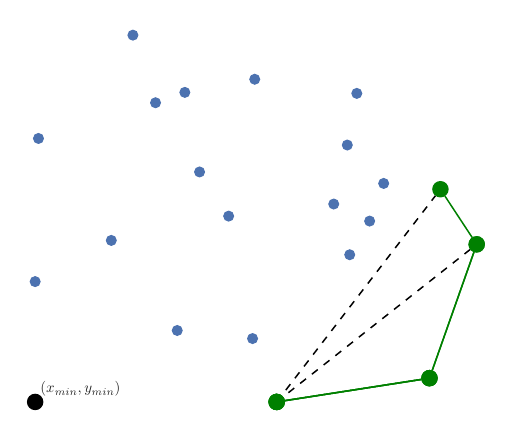
\begin{tikzpicture}[scale=0.9]

\definecolor{darkslategray38}{RGB}{38,38,38}
\definecolor{green}{RGB}{0,128,0}
\definecolor{lightgray204}{RGB}{204,204,204}
\definecolor{steelblue76114176}{RGB}{76,114,176}

\begin{axis}[
axis line style={lightgray204},
hide x axis,
hide y axis,
tick align=outside,
x grid style={lightgray204},
xmajorticks=false,
xmin=0.0669367338947019, xmax=0.894111789939664,
xtick style={color=darkslategray38},
y grid style={lightgray204},
ymajorticks=false,
ymin=-0.0362471743023485, ymax=1.03274876525929,
ytick style={color=darkslategray38}
]
\addplot [semithick, white, mark=*, mark size=3, mark options={solid}]
table {%
0.515872695614497 0.0123435502231805
0.776100950068952 0.0753407526360956
0.856512923755802 0.429885536698643
0.794765500051758 0.575905243509799
0.652331867510728 0.829843579751645
0.271019344924566 0.98415804073376
0.110198245014805 0.710446973195645
0.104535600078564 0.331190264339077
};
\addplot [draw=steelblue76114176, fill=steelblue76114176, mark=*, only marks]
table{%
x  y
0.346517060199814 0.201667385571862
0.110198245014805 0.710446973195645
0.674196381095166 0.49152149407659
0.30956117598126 0.80506608165215
0.271019344924566 0.98415804073376
0.636154602711755 0.693008958661624
0.384544745815431 0.621686927298183
0.613069361293463 0.536676532843469
0.515872695614497 0.0123435502231805
0.856512923755802 0.429885536698643
0.794765500051758 0.575905243509799
0.104535600078564 0.331190264339077
0.698107527894101 0.591287819523784
0.652331867510728 0.829843579751645
0.776100950068952 0.0753407526360956
0.359461819254946 0.832493157115646
0.234215740614521 0.440279847038206
0.474800803395323 0.180277096021146
0.478504950884847 0.867281705269675
0.434092000130053 0.504691515965982
0.640277876553855 0.402360080889356
};
\addplot [semithick, black, mark=*, mark size=3, mark options={solid}]
table {%
0.104535600078564 0.0123435502231805
};
\addplot [semithick, green, mark=*, mark size=3, mark options={solid}]
table {%
0.515872695614497 0.0123435502231805
};
\addplot [semithick, green, mark=*, mark size=3, mark options={solid}]
table {%
0.515872695614497 0.0123435502231805
0.776100950068952 0.0753407526360956
};
\addplot [semithick, green, mark=*, mark size=3, mark options={solid}]
table {%
0.515872695614497 0.0123435502231805
0.776100950068952 0.0753407526360956
0.856512923755802 0.429885536698643
};
\addplot [semithick, dashed, black]
table {%
0.515872695614497 0.0123435502231805
0.856512923755802 0.429885536698643
};
\addplot [semithick, green, mark=*, mark size=3, mark options={solid}]
table {%
0.515872695614497 0.0123435502231805
0.776100950068952 0.0753407526360956
0.856512923755802 0.429885536698643
0.794765500051758 0.575905243509799
};
\addplot [semithick, dashed, black]
table {%
0.515872695614497 0.0123435502231805
0.794765500051758 0.575905243509799
};
\draw (axis cs:0.104535600078564,0.0123435502231805) node[
  scale=0.6,
  anchor=south west,
  text=darkslategray38,
  rotate=0.0
]{$(x_{min}, y_{min})$};
\end{axis}

\end{tikzpicture}

\end{center}
        \onslide<7>% This file was created with tikzplotlib v0.10.1.
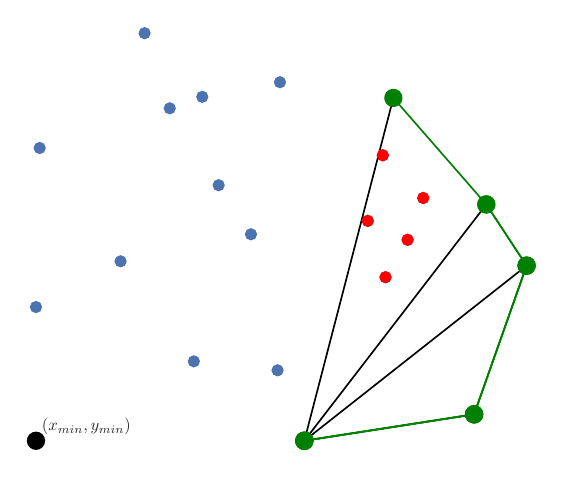
\begin{tikzpicture}

\definecolor{darkslategray38}{RGB}{38,38,38}
\definecolor{green}{RGB}{0,128,0}
\definecolor{lightgray204}{RGB}{204,204,204}
\definecolor{steelblue76114176}{RGB}{76,114,176}

\begin{axis}[
axis line style={lightgray204},
hide x axis,
hide y axis,
tick align=outside,
x grid style={lightgray204},
xmajorticks=false,
xmin=0.0669367338947019, xmax=0.894111789939664,
xtick style={color=darkslategray38},
y grid style={lightgray204},
ymajorticks=false,
ymin=-0.0362471743023485, ymax=1.03274876525929,
ytick style={color=darkslategray38}
]
\addplot [draw=steelblue76114176, fill=steelblue76114176, mark=*, only marks]
table{%
x  y
0.346517060199814 0.201667385571862
0.110198245014805 0.710446973195645
0.674196381095166 0.49152149407659
0.30956117598126 0.80506608165215
0.271019344924566 0.98415804073376
0.636154602711755 0.693008958661624
0.384544745815431 0.621686927298183
0.613069361293463 0.536676532843469
0.515872695614497 0.0123435502231805
0.856512923755802 0.429885536698643
0.794765500051758 0.575905243509799
0.104535600078564 0.331190264339077
0.698107527894101 0.591287819523784
0.652331867510728 0.829843579751645
0.776100950068952 0.0753407526360956
0.359461819254946 0.832493157115646
0.234215740614521 0.440279847038206
0.474800803395323 0.180277096021146
0.478504950884847 0.867281705269675
0.434092000130053 0.504691515965982
0.640277876553855 0.402360080889356
};
\addplot [draw=red, fill=red, mark=*, only marks]
table{%
x  y
0.674196381095166 0.49152149407659
0.636154602711755 0.693008958661624
0.613069361293463 0.536676532843469
0.698107527894101 0.591287819523784
0.640277876553855 0.402360080889356
};
\addplot [semithick, black, mark=*, mark size=3, mark options={solid}]
table {%
0.104535600078564 0.0123435502231805
};
\addplot [semithick, green, mark=*, mark size=3, mark options={solid}]
table {%
0.515872695614497 0.0123435502231805
};
\addplot [semithick, green, mark=*, mark size=3, mark options={solid}]
table {%
0.515872695614497 0.0123435502231805
0.776100950068952 0.0753407526360956
};
\addplot [semithick, green, mark=*, mark size=3, mark options={solid}]
table {%
0.515872695614497 0.0123435502231805
0.776100950068952 0.0753407526360956
0.856512923755802 0.429885536698643
};
\addplot [semithick, black]
table {%
0.515872695614497 0.0123435502231805
0.856512923755802 0.429885536698643
};
\addplot [semithick, green, mark=*, mark size=3, mark options={solid}]
table {%
0.515872695614497 0.0123435502231805
0.776100950068952 0.0753407526360956
0.856512923755802 0.429885536698643
0.794765500051758 0.575905243509799
};
\addplot [semithick, black]
table {%
0.515872695614497 0.0123435502231805
0.794765500051758 0.575905243509799
};
\addplot [semithick, green, mark=*, mark size=3, mark options={solid}]
table {%
0.515872695614497 0.0123435502231805
0.776100950068952 0.0753407526360956
0.856512923755802 0.429885536698643
0.794765500051758 0.575905243509799
0.652331867510728 0.829843579751645
};
\addplot [semithick, black]
table {%
0.515872695614497 0.0123435502231805
0.652331867510728 0.829843579751645
};
\draw (axis cs:0.104535600078564,0.0123435502231805) node[
  scale=0.6,
  anchor=south west,
  text=darkslategray38,
  rotate=0.0
]{$(x_{min}, y_{min})$};
\end{axis}

\end{tikzpicture}

        \onslide<8->\begin{center}
% This file was created with tikzplotlib v0.10.1.
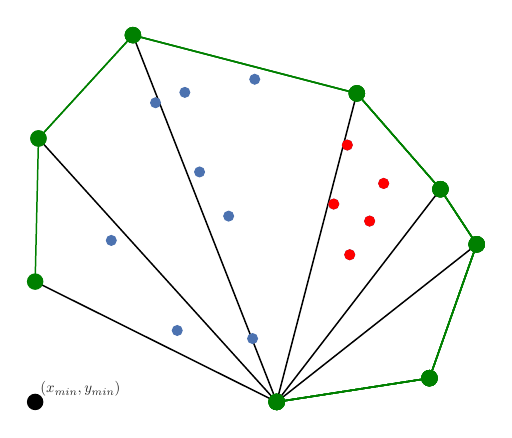
\begin{tikzpicture}[scale=0.9]

\definecolor{darkslategray38}{RGB}{38,38,38}
\definecolor{green}{RGB}{0,128,0}
\definecolor{lightgray204}{RGB}{204,204,204}
\definecolor{steelblue76114176}{RGB}{76,114,176}

\begin{axis}[
axis line style={lightgray204},
hide x axis,
hide y axis,
tick align=outside,
x grid style={lightgray204},
xmajorticks=false,
xmin=0.0669367338947019, xmax=0.894111789939664,
xtick style={color=darkslategray38},
y grid style={lightgray204},
ymajorticks=false,
ymin=-0.0362471743023485, ymax=1.03274876525929,
ytick style={color=darkslategray38}
]
\addplot [draw=steelblue76114176, fill=steelblue76114176, mark=*, only marks]
table{%
x  y
0.346517060199814 0.201667385571862
0.110198245014805 0.710446973195645
0.674196381095166 0.49152149407659
0.30956117598126 0.80506608165215
0.271019344924566 0.98415804073376
0.636154602711755 0.693008958661624
0.384544745815431 0.621686927298183
0.613069361293463 0.536676532843469
0.515872695614497 0.0123435502231805
0.856512923755802 0.429885536698643
0.794765500051758 0.575905243509799
0.104535600078564 0.331190264339077
0.698107527894101 0.591287819523784
0.652331867510728 0.829843579751645
0.776100950068952 0.0753407526360956
0.359461819254946 0.832493157115646
0.234215740614521 0.440279847038206
0.474800803395323 0.180277096021146
0.478504950884847 0.867281705269675
0.434092000130053 0.504691515965982
0.640277876553855 0.402360080889356
};
\addplot [draw=red, fill=red, mark=*, only marks]
table{%
x  y
0.674196381095166 0.49152149407659
0.636154602711755 0.693008958661624
0.613069361293463 0.536676532843469
0.698107527894101 0.591287819523784
0.640277876553855 0.402360080889356
};
\addplot [semithick, black, mark=*, mark size=3, mark options={solid}]
table {%
0.104535600078564 0.0123435502231805
};
\addplot [semithick, green, mark=*, mark size=3, mark options={solid}]
table {%
0.515872695614497 0.0123435502231805
};
\addplot [semithick, green, mark=*, mark size=3, mark options={solid}]
table {%
0.515872695614497 0.0123435502231805
0.776100950068952 0.0753407526360956
};
\addplot [semithick, green, mark=*, mark size=3, mark options={solid}]
table {%
0.515872695614497 0.0123435502231805
0.776100950068952 0.0753407526360956
0.856512923755802 0.429885536698643
};
\addplot [semithick, black]
table {%
0.515872695614497 0.0123435502231805
0.856512923755802 0.429885536698643
};
\addplot [semithick, green, mark=*, mark size=3, mark options={solid}]
table {%
0.515872695614497 0.0123435502231805
0.776100950068952 0.0753407526360956
0.856512923755802 0.429885536698643
0.794765500051758 0.575905243509799
};
\addplot [semithick, black]
table {%
0.515872695614497 0.0123435502231805
0.794765500051758 0.575905243509799
};
\addplot [semithick, green, mark=*, mark size=3, mark options={solid}]
table {%
0.515872695614497 0.0123435502231805
0.776100950068952 0.0753407526360956
0.856512923755802 0.429885536698643
0.794765500051758 0.575905243509799
0.652331867510728 0.829843579751645
};
\addplot [semithick, black]
table {%
0.515872695614497 0.0123435502231805
0.652331867510728 0.829843579751645
};
\addplot [semithick, green, mark=*, mark size=3, mark options={solid}]
table {%
0.515872695614497 0.0123435502231805
0.776100950068952 0.0753407526360956
0.856512923755802 0.429885536698643
0.794765500051758 0.575905243509799
0.652331867510728 0.829843579751645
0.271019344924566 0.98415804073376
};
\addplot [semithick, black]
table {%
0.515872695614497 0.0123435502231805
0.271019344924566 0.98415804073376
};
\addplot [semithick, green, mark=*, mark size=3, mark options={solid}]
table {%
0.515872695614497 0.0123435502231805
0.776100950068952 0.0753407526360956
0.856512923755802 0.429885536698643
0.794765500051758 0.575905243509799
0.652331867510728 0.829843579751645
0.271019344924566 0.98415804073376
0.110198245014805 0.710446973195645
};
\addplot [semithick, black]
table {%
0.515872695614497 0.0123435502231805
0.110198245014805 0.710446973195645
};
\addplot [semithick, green, mark=*, mark size=3, mark options={solid}]
table {%
0.515872695614497 0.0123435502231805
0.776100950068952 0.0753407526360956
0.856512923755802 0.429885536698643
0.794765500051758 0.575905243509799
0.652331867510728 0.829843579751645
0.271019344924566 0.98415804073376
0.110198245014805 0.710446973195645
0.104535600078564 0.331190264339077
};
\addplot [semithick, black]
table {%
0.515872695614497 0.0123435502231805
0.104535600078564 0.331190264339077
};
\draw (axis cs:0.104535600078564,0.0123435502231805) node[
  scale=0.6,
  anchor=south west,
  text=darkslategray38,
  rotate=0.0
]{$(x_{min}, y_{min})$};
\end{axis}

\end{tikzpicture}

\end{center}
      \end{overprint}
    \end{figure}
  \end{center}

  \begin{overprint}
    \onslide<9>{
      \begin{equation}
        \text{Custo} = \underbrace{h}_{\text{Região convexa}} \times (\underbrace{O(n)}_{\text{Próximo Ponto}} + \underbrace{O(n)}_{\text{Pontos dentro}}) = O(hn)
      \end{equation}
    }
  \end{overprint}
\end{frame}

\begin{frame}{Exemplos}

  \begin{overprint}
    \begin{columns}
      \begin{column}{0.5\textwidth}
        \begin{figure}
          \includegraphics<1-2>[width=\textwidth]{./figures/introbs_pointsonly.png}
          \includegraphics<3-4>[width=\textwidth]{./figures/fishdp_pointsonly.png}
          \includegraphics<5-6>[width=\textwidth]{./figures/dog_pointsonly.png}
          \includegraphics<7-8>[width=\textwidth]{./figures/canada_pointsonly.png}
        \end{figure}
      \end{column}
      \begin{column}{0.5\textwidth}
        \begin{figure}
          \includegraphics<2>[width=\textwidth]{./figures/introbs.png}
          \includegraphics<4>[width=\textwidth]{./figures/fishdp.png}
          \includegraphics<6>[width=\textwidth]{./figures/dog.png}
          \includegraphics<8>[width=\textwidth]{./figures/canada.png}
        \end{figure}
      \end{column}
    \end{columns}
  \end{overprint}

\end{frame}

\begin{frame}
\frametitle{Tempo de execução}
  \begin{itemize}
    \item Pontos gerados aleatoriamente dentro de um círculo de raio 1
    \item $h \sim \sqrt{n}$
  \end{itemize}
\end{frame}

\begin{frame}
\frametitle{Tempo de execução}
% Two columns
\begin{columns}
  \begin{column}{0.7\textwidth}
    \begin{figure}
      \includegraphics[width=0.9\textwidth]{./figures/circles_time.png}
    \end{figure}
  \end{column}
  \begin{column}{0.3\textwidth}
    Pontos gerados aleatoriamente no intervalo dentro de um círculo.
  \end{column}
\end{columns}
\end{frame}

\end{document}
